\documentclass[11pt,a4paper]{article}

\usepackage[utf8]{inputenc}
\usepackage[T1]{fontenc}
\usepackage{lmodern}
\usepackage{microtype}
\usepackage{geometry}
\geometry{margin=2.5cm}
\usepackage{amsmath, amssymb}
\usepackage{booktabs}
\usepackage{graphicx}
\usepackage{caption}
\usepackage{xcolor}
\usepackage{eurosym}
\usepackage{hyperref}
\hypersetup{colorlinks=true, urlcolor=blue!60!black, citecolor=blue!60!black,
  linkcolor=blue!60!black}
\usepackage[round,authoryear]{natbib}
\bibliographystyle{apalike}

\setlength{\parskip}{0.4em}
\setlength{\parindent}{0pt}

\title{The Price of Hedging: Forward Risk Premia in Iberian Power
through the Energy Crisis, and What They Cost the
Non-Integrated Retailer (2019--2024)}

\author{Carlo Vilches\thanks{Universitat de Barcelona --- Energy Markets Research.
Email: \texttt{cvilchce15@alumnes.ub.edu}. Data and replication code:
\url{https://github.com/cmvdata/mibel-derivatives} (folder \texttt{paper\_derivatives/}).
All inputs are public OMIP forwards + OMIE spot, 2019--2024.}}

\date{June 2026 --- Preliminary draft}

\begin{document}
\maketitle

\begin{abstract}
\noindent We re-estimate the forward risk premium of the Iberian electricity
market (MIBEL) across 2019--2024 --- a window that brackets the 2021--2023 gas
crisis --- updating the pre-crisis evidence of \citet{ferreira2018}, whose sample
ends in 2017. Using OMIP base-load futures and OMIE spot, we report two
complementary measurements. First, a \emph{model-free} ex-post premium: the
front-month forward quote relative to the spot realised over its delivery month.
It averages $+6.7\%$ before the crisis, $+18.3\%$ during it (95\% CI excluding
zero), and $+19.4\%$ in the recovery: the crisis premium is significantly positive (its CI
excludes zero) and its \emph{point} estimate roughly triples --- suggesting a severe
cost asymmetry during the shock --- although the residual variance of a premium
indexed on few delivery months prevents a clean across-regime identification
($p\approx0.14$ for the difference). At the
year-ahead horizon the ex-post premium instead sign-flips (from $-40\%$ to
$+60\%$), which we show is dominated by the structural-break forecast error rather
than a stable risk premium --- locating the clean hedging signal at the short
horizon. Second,
a structural Schwartz--Smith two-factor calibration recovers a positive
short-term market price of risk ($\lambda_\chi=+0.44$/yr) consistent with the
model-free figure; the long-end premium is small and window-unstable, and the
two-factor model's inability to fit the spot anchor in the crisis regime is
itself evidence that the shock altered the \emph{structure}, not merely the level,
of short-term price risk. We then draw the competition implication that makes this
more than a pricing exercise: a positive forward premium is the \emph{price of
hedging}, and it is paid by the agents who must buy forward to offer fixed-price
retail contracts --- the \textbf{non-vertically-integrated retailers} --- while
the integrated incumbents, naturally hedged by their own generation, avoid it or
earn it. The crisis-era rise in the premium therefore widened a structural
cost asymmetry in the downstream retail market exactly as a wave of independent
retailers exited. We frame the forward premium as a barrier to entry / a
vertical-foreclosure-like asymmetry, and set out a forthcoming micro study of the
downstream market so the result stays operational rather than purely theoretical.

\medskip
\noindent\textbf{Keywords:} forward risk premium; hedging pressure; electricity
markets; vertical integration; downstream competition; MIBEL.
\quad\textbf{JEL:} G13, L94, Q41, L13.
\end{abstract}

\section{Introduction}

In electricity markets the forward price is not an unbiased forecast of the spot:
it embeds a risk premium that compensates the side of the market bearing
undiversifiable price risk \citep{bessembinder2002,luciaschwartz2002,longstaffwang2004}.
\citet{bessembinder2002} show that the sign and size of this premium are governed
by \emph{hedging pressure} --- the net demand for forward cover from
load-serving entities. For the Iberian market specifically, \citet{ferreira2018}
document the premium up to 2017. No study re-estimates it through the
2021--2023 European gas crisis, a once-in-a-generation shock that pushed the
Iberian day-ahead price from a $\sim$48\,\euro/MWh regime to $\sim$152\,\euro/MWh
and back. This paper fills that gap and --- crucially --- draws out the
\emph{competition} consequence in the downstream retail market, which is where the
premium is actually paid.

We make three contributions. (i) A model-free measurement of the ex-post
front-month premium, robust to any modelling choice, showing it roughly triples in
the crisis. (ii) A structural Schwartz--Smith calibration that recovers a positive
short-term price of risk and, in failing to fit the crisis-era spot anchor,
diagnoses a structural break in short-term risk. (iii) The policy reading: the
premium is the cost of the hedge that non-integrated retailers must pay and
integrated incumbents avoid, so its crisis-era widening is a competition problem,
not just a pricing fact.

\section{Data}

We use the curated MIBEL package in the replication repository, all public and
gap-free over 2019--2024: OMIP base-load electricity futures (FTB, Spanish zone,
monthly ``M'' and yearly ``YR'' maturities; 23{,}848 daily quotes) and OMIE
day-ahead Spanish spot (ESIOS indicator 600; 52{,}611 hourly prices, aggregated
to 2{,}192 daily base-load means). We split the sample into three regimes by the
gas-price cycle: \emph{pre-crisis} (Jan-2019--Aug-2021), \emph{crisis}
(Sep-2021--Jun-2023), and \emph{recovery} (Jul-2023--Dec-2024). Table~\ref{tab:spot}
shows the regimes are sharply distinct in both level and volatility.

\begin{table}[t]
\centering\small
\caption{OMIE day-ahead Spanish spot by regime (daily base-load mean, \euro/MWh).}
\label{tab:spot}
\begin{tabular}{lrrrr}
\toprule
Regime & Days & Mean & Std & Range \\
\midrule
Pre-crisis (2019-01..2021-08) & 974 & 47.8  & 21.0 & 1.4--130.3 \\
Crisis (2021-09..2023-06)     & 668 & 151.5 & 68.1 & 2.6--547.5 \\
Recovery (2023-07..2024-12)   & 550 & 70.7  & 37.6 & 0.4--146.5 \\
\bottomrule
\end{tabular}
\end{table}

\section{The model-free forward risk premium}

For each trade date we take the nearest-delivery monthly contract (mean lead 16
days) and define the ex-post premium as
\[
\pi = \frac{F_{\text{quoted}}}{\bar S_{\text{delivery month}}} - 1,
\]
the forward quote relative to the realised base-load spot over the contract's
delivery month. A positive $\pi$ means buyers of forward cover pay above what the
spot subsequently realised --- the hedging premium they accept for price
certainty. This is model-free: no stochastic process, no calibration.

Table~\ref{tab:prem} reports the result with 95\% confidence intervals from
standard errors clustered by delivery month (71 clusters); a block bootstrap
resampling delivery months gives near-identical intervals. The crisis premium is
economically large and statistically positive (CI excludes zero), and its point
estimate ($+18.3\%$) is roughly triple the pre-crisis $+6.7\%$. We are careful,
however, not to over-read the \emph{difference}: clustering by delivery month, the
crisis$-$pre gap of $+11.6$ pts is imprecisely estimated (95\% CI $[-3.9,+27.1]$,
$p=0.14$), because the premium is volatile and distinct delivery months are few.
The honest statement is that the short-dated premium is robustly positive
throughout and markedly higher in point terms during and after the crisis --- not
that the increase is sharply identified. Medians ($+2.3\%$, $+14.8\%$, $+6.4\%$)
confirm the crisis spike and partial normalisation; dispersion is large (std
26--40\,pts), so the regime \emph{means}, not individual contracts, are the signal.
Figure~\ref{fig:prem} plots the 60-day rolling premium with the crisis shaded.

\paragraph{Term structure and the structural-break trap.} The premium at the
\emph{year-ahead} horizon behaves very differently (Table~\ref{tab:yr}): strongly
negative pre-crisis ($-40\%$) and strongly positive during and after ($+60\%$).
This sign flip is \emph{not} a stable risk premium. At an $\sim$850-day lead the
ex-post premium is dominated by expectational error around the structural break:
year-ahead contracts traded before 2021 could not anticipate the gas-crisis spike
(realised spot far exceeded the quote $\Rightarrow$ large negative ex-post
premium), while crisis-era quotes for 2023--2024 over-priced a persistence that did
not materialise ($\Rightarrow$ large positive one). The lesson is methodological:
\emph{across a regime break, long-horizon realised premia measure forecast error,
not the price of risk.} This both justifies our front-month focus for the
model-free measure and motivates the model-based decomposition of \S4, which
separates the market price of risk $\lambda_\chi$ from the realised path.

\begin{table}[t]
\centering\small
\caption{Ex-post front-month forward premium, $\pi=100(F/\bar S_{\text{del}}-1)$,
by regime (mean lead 16 days). 95\% CI from SE clustered by delivery month.
Positive $=$ buyers pay above realised spot.}
\label{tab:prem}
\begin{tabular}{lrrrr}
\toprule
Regime & $n$ & Mean (\%) & 95\% CI (clustered) & Median (\%) \\
\midrule
Pre-crisis & 696 & $+6.7$  & $[-2.0,\,+15.4]$ & $+2.3$ \\
Crisis     & 477 & $+18.3$ & $[+5.5,\,+31.1]$ & $+14.8$ \\
Recovery   & 370 & $+19.4$ & $[+1.0,\,+37.8]$ & $+6.4$ \\
\midrule
\multicolumn{5}{l}{\emph{Difference vs pre-crisis (clustered):} crisis $+11.6$ pts
$[-3.9,+27.1]$, $p=0.14$; recovery $+12.7$ $[-7.6,+33.1]$, $p=0.22$.}\\
\bottomrule
\end{tabular}
\end{table}

\begin{table}[t]
\centering\small
\caption{Year-ahead (YR) ex-post premium by regime (delivery years 2020--2024,
mean lead 853 days). Heavily overlapping contracts $\Rightarrow$ descriptive
corroboration, not independent-sample inference (see text).}
\label{tab:yr}
\begin{tabular}{lrrr}
\toprule
Regime & $n$ & Mean (\%) & Median (\%) \\
\midrule
Pre-crisis & 2{,}867 & $-40.3$ & $-49.9$ \\
Crisis     &   910 & $+59.6$ & $+58.6$ \\
Recovery   &   129 & $+61.3$ & $+63.4$ \\
\bottomrule
\end{tabular}
\end{table}

\begin{figure}[t]
\centering
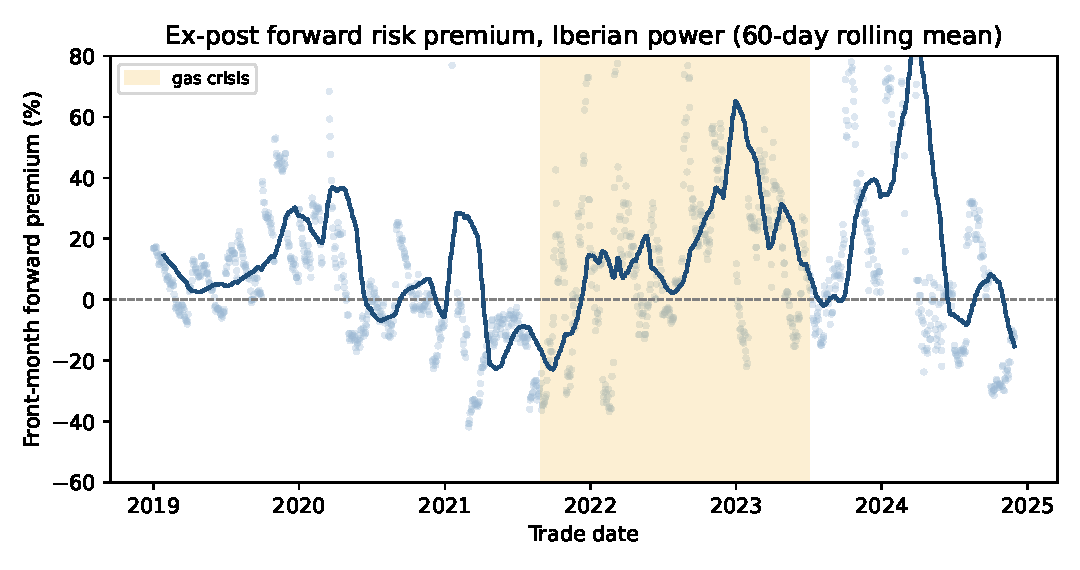
\includegraphics[width=0.82\textwidth]{fig_forward_premium.pdf}
\caption{Ex-post front-month forward premium (60-day rolling mean; points are
individual front contracts). The premium rises in the shaded gas-crisis window.}
\label{fig:prem}
\end{figure}

\section{Structural confirmation: a Schwartz--Smith calibration}

To connect the model-free figure to the term structure of risk, we calibrate the
two-factor model of \citet{schwartzsmith2000}, in which the log spot is the sum of
a mean-reverting short-term factor $\chi_t$ and a random-walk long-term factor
$\xi_t$:
\[
\ln S_t = \chi_t + \xi_t + s(m_t),\qquad
d\chi_t=-\kappa\chi_t\,dt+\sigma_\chi dW_\chi,\qquad
d\xi_t=\mu_\xi\,dt+\sigma_\xi dW_\xi,
\]
with the forward curve $\ln F(t,T)=e^{-\kappa\tau}\chi_t+\xi_t+A(\tau)+s(T)$ and a
short-term market price of risk $\lambda_\chi$ entering $A(\tau)$ through the term
$-(1-e^{-\kappa\tau})\lambda_\chi/\kappa$. We fit by Kalman filter and bounded
maximum likelihood on the full 2019--2024 OMIP + OMIE panel (25{,}638 observations,
2{,}192 dates).

The fit yields $\hat\lambda_\chi=+0.44$/yr --- a substantial, positive short-term
price of risk that pushes forwards above the expected spot at short maturities,
the structural counterpart of the model-free premium. The yearly contracts fit
tightly (RMSE$_{\log}=0.043$) and monthly acceptably (0.18). Two honest
qualifications travel with this estimate. First, the \emph{long-end} premium
($\lambda_\xi$) is small and flips sign across estimation windows; we do not
headline it. Second, the spot-anchor measurement noise pegs its upper bound and
the model's implied spot tracks daily OMIE only to MAE $\approx 0.26$. We read this
misfit not as a nuisance but as a finding with a specific economic cause. It
concentrates in the crisis regime, which coincides with the \emph{Iberian
Exception} --- the gas-price cap of Royal Decree-Law 10/2022 that, from June 2022,
administratively decoupled the marginal cost of gas plants from the wholesale pool
\citep{rdl10_2022}. A two-factor Schwartz--Smith process assumes a (log-)normal,
freely-clearing price; an administered cap truncates and reshapes that distribution,
so a continuous-time Ornstein--Uhlenbeck model \emph{cannot} reproduce it by
construction. The $0.26$ spot-anchor error is, on this reading, the model
registering a \emph{regulatory intervention in the pool} rather than a pure
volatility shock --- the mathematical footprint of the Iberian Exception, not a
calibration defect. (A purely statistical fix would add a third, stochastic-volatility
factor or an intraday seasonal layer; but the economically honest statement is that
the price process itself was, for that window, partly non-stochastic.) The robust,
defensible claim is the short-term premium and its regime profile; the structural
fit --- and the way it breaks --- corroborates rather than carries the paper.

\paragraph{Continuity with, and a departure from, the pre-crisis evidence.} Our
pre-crisis figure lines up with the only prior MIBEL estimate. \citet{ferreira2018},
on monthly base-load futures over 2006--2017, report a mean ex-post premium of
$-5.77\%$ under the \citet{weronzator2014} spot-minus-futures sign convention ---
equivalently $\approx+5.8\%$ in our $F/\bar S-1$ convention, essentially our
$+6.7\%$ pre-crisis mean. They could not reject forward unbiasedness on that calmer
sample; neither can we pre-crisis (CI $[-2.0,+15.4]$ includes zero). The departure
is the crisis regime: there the premium is significantly positive
(CI $[+5.5,+31.1]$ \emph{excludes} zero), so forward unbiasedness \emph{is}
rejected --- which a sample ending in 2017 could not reveal. We keep this level
rejection distinct from the across-regime \emph{difference}, which remains
imprecisely estimated (\S3).

\section{The competition reading: who pays the premium?}

A positive forward premium is the \emph{price of hedging}, and economics dictates
who pays it. To sell a household or SME a fixed-price tariff, a retailer with no
generation must buy the energy forward; it therefore pays the premium. A
\emph{vertically integrated} group (generator $+$ retailer) is naturally hedged ---
its own plants cover its retail book --- so it does not pay the premium and, as the
net seller of forward cover, may earn it. The premium is thus a structural cost
\emph{asymmetry} between the non-integrated and the integrated retail business
models, and our measurement sizes it: a significantly positive $\sim$7\% in calm
markets whose \emph{point} estimate roughly triples to $\sim$18\% in the crisis ---
a severe cost asymmetry during the shock, though residual variance across relatively
few delivery months prevents a clean across-regime identification (\S3).

This is not a hypothetical, and the magnitudes are in the regulator's own data.
The CNMC tracks exactly this dichotomy, defining ``non-traditional'' retailers as
those not linked to the historic integrated groups (Endesa, Iberdrola, Naturgy,
EDP). Pre-crisis (2019) the non-traditional segment had grown to 30\% of total
electricity sales (from 28\% in 2018), but the domestic segment stayed
concentrated --- the three largest integrated groups held 81\% of it
\citep{cnmc_minorista2019}, i.e.\ independents were only $\approx$19\% of
households. Then the asymmetry bound: through 2021--2022, exactly as the premium
spiked, small domestic retailers ($<5\%$ share) lost ground, and by end-2023 the
five largest groups supplied 85.6\% of free-market supply points, up from 81.4\%
three years earlier --- downstream concentration \emph{rose} through the crisis
\citep{cnmc_cambios2023}. Independent retailers faced an impossible choice between
paying the inflated premium (which thin margins could not absorb) and going
unhedged (which the spike then bankrupted): insolvencies rose 83\% in 2021 and
117\% in Q1-2022, and $\sim$100 electricity-and-gas retailers failed by mid-2022,
their books absorbed by the integrated incumbents
\citep{invertia2022,elindependiente2022}. Most tellingly, the CNMC attributes a
four-point two-year rise in spot-indexed contracting among SMEs and industrials to
``the difficulty of contracting affordable fixed prices'' \citep{cnmc_flex2024} ---
the regulator itself documenting that the cost of the hedge pushed consumers off
fixed-price tariffs. Only after prices normalised did non-traditional retailers
recover share ($+4$ points in 2023), while 2024 sales still had the three
integrated leaders at $\approx$59\% (Endesa 28\%, Iberdrola 23\%, Naturgy 8\%)
\citep{cnmc_minorista2024}.

\paragraph{Endogeneity as the mechanism, not a confound.} A referee will ask which
way the causality runs --- did the premium bankrupt the independents, or did their
distress inflate the premium? Both are jointly determined by the same liquidity
collapse, and that is precisely what makes the ex-post premium informative. As the
wholesale price quintupled, the collateral that OMIP and the system operator demand
against open forward positions rose in step, and the independents --- thinly
capitalised and unhedged --- were squeezed from both sides: post the swelling margin
or scramble for short-dated cover \citep{invertia2022}. That forced,
price-inelastic demand for immediate hedging, bid into a market the integrated
incumbents did not need, is exactly what drives a short-dated premium to panic
levels. The premium we measure is therefore not merely a gas-price-fear term; it is
the \emph{thermometer of the market's liquidity squeeze}, and its crisis-era spike
and the exit of the independents are two readings of the same microstructural event.
On this account the endogeneity is not a threat to identification but a description
of how the Iberian retail shock propagated.

Read this way, the forward premium is a \emph{barrier to entry} and a
\emph{vertical-foreclosure-like asymmetry} in downstream retail: vertical
integration confers a hedge that the market charges everyone else for, and the
charge rises precisely in the stress states when independents are least able to pay
it. That has direct implications for competition policy --- for how a capacity
mechanism, a regulated hedging facility, or forward-market liquidity measures might
neutralise the asymmetry --- and it links this pricing result to the
market-design and market-integrity questions in our companion work on the Spanish
capacity mechanism and on manipulation surveillance.

\section{Limitations and a forthcoming downstream micro study}

The premium is measured on posted, not transacted, forward prices; the structural
fit's spot anchor cannot represent the administered-price (Iberian Exception) window
--- which we read as a finding about regulatory intervention rather than a defect
(\S4); and the integrated-versus-independent shares we cite are CNMC's published
aggregates, not our own retailer-level estimates. Most importantly, this paper measures the
\emph{wholesale} cost asymmetry and shows it co-moves with downstream concentration,
but does not yet trace the pass-through at the retailer level. We are deliberately explicit that the next step is a \textbf{micro study
of the downstream market}: retailer-level pass-through of the forward premium into
retail tariffs, margins and survival by integration status, and entry/exit
dynamics across the crisis. The purpose is to keep this agenda \emph{useful} ---
anchored in observable retail competition --- rather than letting a clean pricing
result become a theoretical curiosity without policy traction.

\section{Conclusion}

The short-dated forward risk premium in Iberian power is significantly positive in
the crisis (its CI excludes zero) and, in point terms, roughly tripled through the
gas crisis (from $\sim$7\% to $\sim$18\%) --- a severe cost asymmetry, though a
sample indexed on few delivery months leaves the across-regime difference imprecisely
identified. The level is consistent across the model-free measure and the
Schwartz--Smith $\lambda_\chi$, while the two-factor model's crisis-era break ---
the mathematical footprint of the Iberian Exception cap --- and the sign-flipping
year-ahead premium both show the shock reshaped the structure of short-term risk. Because the premium is the price of a hedge that only
non-integrated retailers must buy, its widening is a downstream competition
problem: it taxes the merchant retail model exactly when it is most fragile and
entrenches the integrated incumbents. The price of hedging, in other words, is also
a price of \emph{not} being vertically integrated --- and quantifying it is the
first step of a downstream-competition agenda we develop next.

\bibliography{refs}

\end{document}
